\section{Information loss and decision-relevant state}\label{sec:C02:02}
Let $H$ denote interaction history and $Z=\varphi(H)$ a compressed representation. Compression is useful when decisions can be made from $Z$ with acceptable loss. Faithful text reconstruction is only one possible objective. A task may require preserving an authorization expiry time while allowing substantial paraphrase of everything else. Conversely, a summary with high lexical similarity may lose precisely the condition that changes the correct action.

For a discrete future target $Y$ with finite relevant conditional entropies, the Bayes-optimal log-loss using history is $H(Y\mid H)$ and using the compressed representation is $H(Y\mid Z)$. For deterministic $Z=\varphi(H)$,
\begin{align}
 H(Y\mid Z)-H(Y\mid H)
 &=I(Y;H\mid Z)\geq0.
 \label{eq:c02:informationgap}
\end{align}
This follows by expanding conditional mutual information and using that conditioning on $(H,Z)$ is equivalent to conditioning on $H$. Equality characterizes sufficiency for that target. It does not establish sufficiency for a different target, a changed objective, or a new tool interface. A representation optimized for next-token prediction may discard information needed for a rare future intervention.

The relevant target for control can be the optimal action, a value function, a constraint event, or a predictive distribution over consequences. These targets need not agree. Consider a binary historical fact $B$ that has negligible effect on the average continuation text but determines whether a destructive operation is permitted. A compression objective dominated by common conversational tokens can tolerate losing $B$, while a risk-sensitive action objective cannot. This is a decision-theoretic explanation for evaluating compaction through subsequent behavior rather than summarization quality alone.

Define the Bayes decision risk for representation $Z$ and loss $\ell$ by
\begin{equation}
 R^*(Z)=\inf_d\mathbb E[\ell(d(Z),Y)].
\end{equation}
Because every decision rule on $Z$ is also a decision rule on $H$, $R^*(H)\leq R^*(Z)$. The inequality is distribution-specific. It provides no numerical guarantee without assumptions on the lost information and the loss. A practical approximation is to train or evaluate a family of decision probes, including rare constraints, temporal updates, and adversarial distractors. Passing those probes constrains failure in the tested family; it does not prove universal sufficiency.

\subsection{A bounded decision-loss consequence}\label{sec:C02:riskbound}
Assume finite decision and target spaces, $Z=\varphi(H)$, and a fixed loss $0\leq\ell(a,y)\leq L_{\max}$. Write $Q_h=P(Y\in\cdot\mid H=h)$ and $Q_z=P(Y\in\cdot\mid Z=z)$.
\begin{equation}
 f(Q)=\min_a\mathbb E_Q\ell(a,Y),\qquad
 \operatorname{TV}(P,Q)=\sup_B|P(B)-Q(B)|.
\end{equation}
The conditional Bayes risks satisfy $R^*(H)=\mathbb E f(Q_H)$ and $R^*(Z)=\mathbb E f(Q_Z)$. For any $P,Q$, using an optimizer for one distribution as a candidate for the other and then exchanging their roles gives
\begin{equation}
 |f(P)-f(Q)|\leq L_{\max}\operatorname{TV}(P,Q).
\end{equation}
Consequently, with natural logarithms and finite conditional mutual information,
\begin{equation}
\begin{aligned}
 0\leq R^*(Z)-R^*(H)
 &\leq L_{\max}\mathbb E\operatorname{TV}(Q_H,Q_Z)\\
 &\leq L_{\max}\sqrt{\tfrac12\mathbb E\operatorname{KL}(Q_H\Vert Q_Z)}\\
 &=L_{\max}\sqrt{\tfrac12 I(Y;H\mid Z)}.
\end{aligned}
\end{equation}
The first inequality uses that a rule on $Z$ is available to the decision maker observing $H$. The next steps use the bounded-loss variational inequality, Pinsker's inequality and Jensen's inequality~\cite{ch02_reid2011}. The right side can be capped at $L_{\max}$. If information is measured in bits, replace $I$ by $(\log 2)I$. This is a bound on the Bayes-optimal representation gap, not on the actual deployed policy. For a realized decision rule $d_Z$,
\begin{equation}
 \mathbb E\ell(d_Z(Z),Y)-R^*(H)
 =[R^*(Z)-R^*(H)]+[\mathbb E\ell(d_Z(Z),Y)-R^*(Z)].
\end{equation}
The second term is the remaining decision-rule regret and is not controlled by the information bound. The target, loss, task distribution and decision space must remain fixed. A small average bound for one target does not certify a rare permission constraint or the truth of an effect ledger. Those remain distinct from the proposal-preservation, authority and effect contracts in Chapter~\ref{ch:C01}.

Figure~\ref{fig:C02:aliasing} exhibits the complementary pointwise obstruction. If two histories with distinct unique conditional optima collapse to one representation, a deterministic rule with only that representation cannot be optimal for both. A strict population risk increase additionally requires positive probability and positive excess loss on the affected histories or regions.
\begin{figure}[!htbp]
\centering
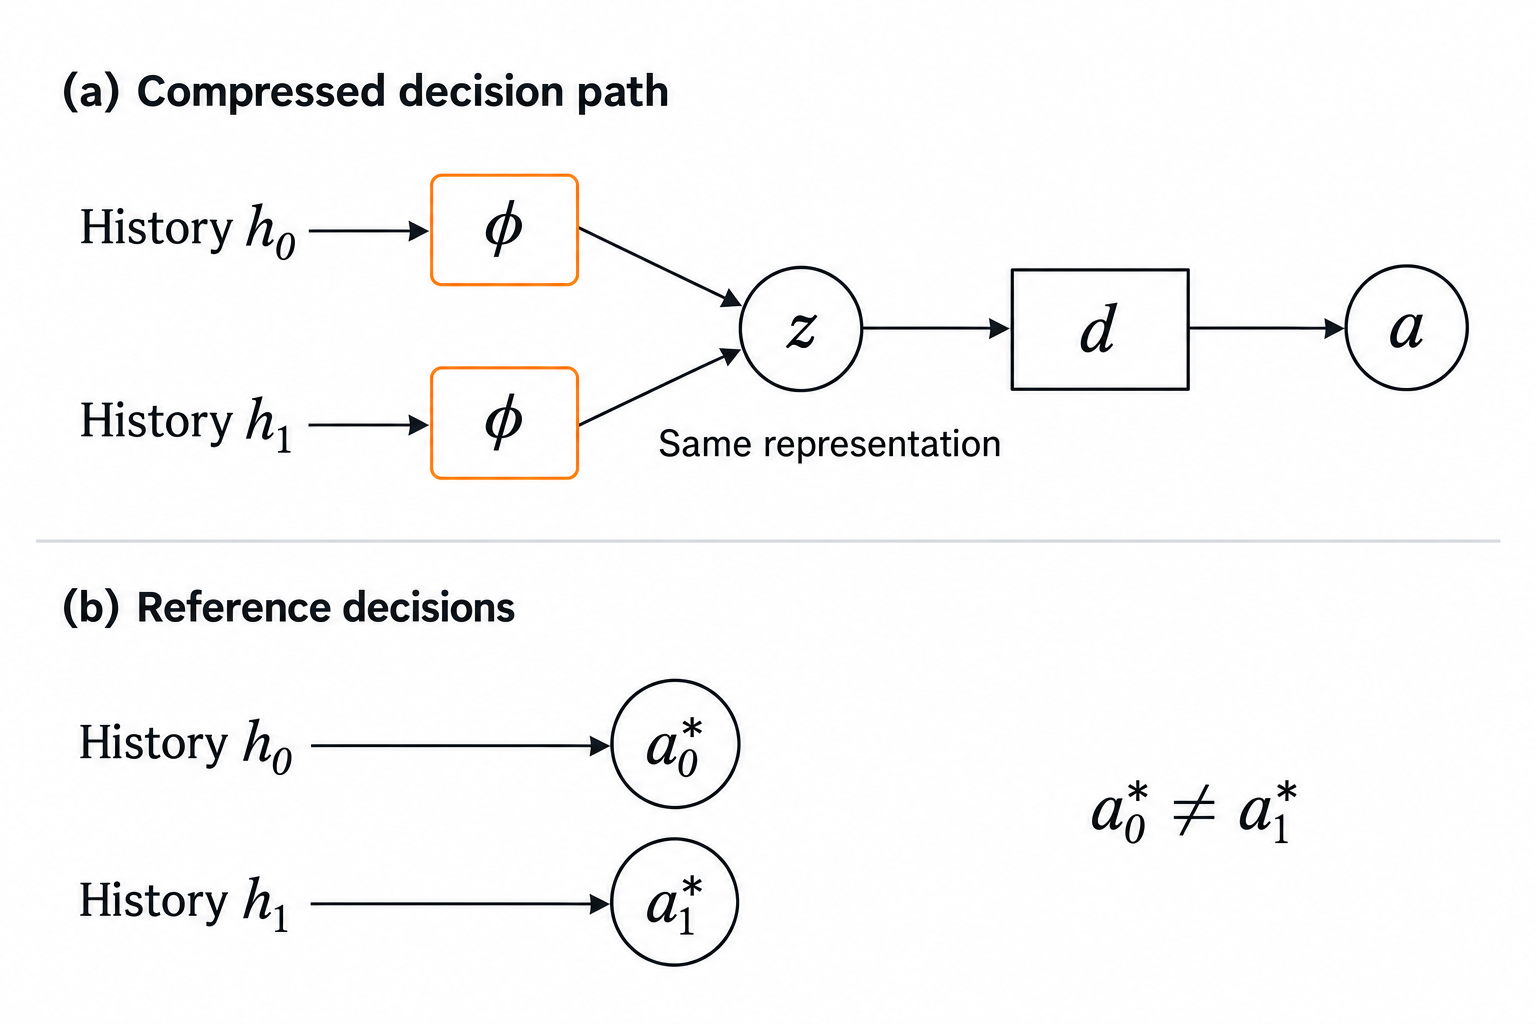
\includegraphics[width=\linewidth]{book/figures/assets/F02v2.png}
\caption{Representation aliasing is target-dependent. Distinct histories $h_0,h_1$ satisfy $\varphi(h_0)=\varphi(h_1)=z$, so a deterministic rule using only $z$ returns the same $a=d(z)$. Under a declared loss with different unique conditional optimal actions $a_0^*,a_1^*$, that action cannot be optimal for both histories. This analytical construction contains no measurements; it does not quantify a population risk gap or exclude policies acquiring additional evidence.}
\label{fig:C02:aliasing}
\end{figure}

Rate-distortion language makes the resource tradeoff explicit:
\begin{equation}
 \min_{p(z\mid h)} I(H;Z)
 \quad\text{subject to}\quad
 \mathbb E[\mathfrak d(H,Z)]\leq\epsilon.
\end{equation}
For agents, a useful distortion $\mathfrak d$ should reflect decision loss or violated constraints. Token count is a proxy for representation cost, not mutual information itself. External memory also changes the problem: a compact working state can defer details to a store, but only if future retrieval is reliable and affordable. The combined representation is then the active state plus the retrieval mechanism, not the summary in isolation~\cite{packer2023memgpt,lewis2020rag}.


If retrieval remains available, the decision experiment must specify its query policy, store version, observation channel, and cost. It then compares information-acquisition systems, rather than the one-shot risks of two representations under an unchanged information set.
